% Embedded Systems lab report -- compile with pdflatex (twice, for the ToC)
\documentclass[11pt,a4paper]{article}

\usepackage[margin=2.5cm]{geometry}
\usepackage{lmodern}      % scalable Type1 fonts for T1; without this,
\usepackage[T1]{fontenc}  % MiKTeX builds slow, fuzzy METAFONT bitmaps
\usepackage[utf8]{inputenc}
\usepackage{amsmath}
\usepackage{graphicx}
\usepackage{float}
\usepackage{array}
\usepackage{booktabs}
\usepackage{xcolor}
\usepackage{listings}
\usepackage{tikz}
\usetikzlibrary{positioning,arrows.meta}
\usepackage[hidelinks]{hyperref}

% --- C code listing style -------------------------------------------------
\definecolor{codegray}{gray}{0.96}
\definecolor{codegreen}{rgb}{0.0,0.5,0.0}
\definecolor{codeblue}{rgb}{0.0,0.0,0.6}

\lstdefinestyle{cstyle}{
  language=C,
  backgroundcolor=\color{codegray},
  basicstyle=\ttfamily\footnotesize,
  keywordstyle=\color{codeblue}\bfseries,
  commentstyle=\color{codegreen}\itshape,
  stringstyle=\color{red!70!black},
  numbers=left,
  numberstyle=\tiny\color{gray},
  numbersep=8pt,
  breaklines=true,
  frame=single,
  framerule=0pt,
  showstringspaces=false,
  tabsize=4,
  captionpos=b,
}
\lstdefinestyle{plain}{
  language={},
  backgroundcolor=\color{codegray},
  basicstyle=\ttfamily\footnotesize,
  numbers=none,
  breaklines=true,
  frame=single,
  framerule=0pt,
  captionpos=b,
}
\lstset{style=cstyle}

\setlength{\emergencystretch}{2em}

% --- Title ----------------------------------------------------------------
\newcommand{\studentid}{R12942157}

\title{Embedded Systems Laboratory Report\\
       \large Digital Filtering of Sensor Data with CMSIS-DSP and CMSIS-RTOS2\\
       \normalsize Basic Problem and Option Problem 1}
\author{YU-CHEN, CHU\\
        \normalsize Student ID: \studentid}
\date{\today\\[2ex]
      \normalsize Source code:
      \url{https://github.com/oldpig123/embedded_system/tree/master/lab7}}

\begin{document}
\maketitle
\tableofcontents
\newpage

% =========================================================================
\section{Introduction}

CMSIS-DSP is Arm's signal processing library for Cortex-M processors. It
contains filters, transforms, statistics and matrix functions, with versions
that use the DSP instructions and the floating-point unit (FPU) of the
Cortex-M4.

The basic problem asks for a DSP program that processes data from a sensor on
the STM32 IoT node. I chose the accelerometer and a finite impulse response
(FIR) low-pass filter. Before I used real data, I tested the program with a
known signal. This test is the \texttt{arm\_fir\_example} from the lecture:
a 1\,kHz plus 15\,kHz input with a reference output that MATLAB computed.

Option problem~1 puts the same processing into three CMSIS-RTOS2 tasks. The
first task reads the sensor when a timer triggers it. The second task filters
the data. The third task sends the raw and the filtered data over Wi-Fi to a
PC, which plots both.

% =========================================================================
\section{Environment}

\begin{table}[h]
\centering
\caption{Hardware and software.}
\begin{tabular}{@{}lp{11.5cm}@{}}
\toprule
Board            & B-L475E-IOT01A (STM32L475VG, Cortex-M4F, 80\,MHz) \\
Sensor           & LSM6DSL accelerometer on I2C2, read with the board support package (BSP) \\
Configuration    & STM32CubeMX 6.18.1, STM32Cube FW\_L4 V1.18.2 (HAL) \\
DSP library      & CMSIS-DSP V1.6.0, prebuilt \texttt{libarm\_cortexM4lf\_math.a} (little endian, hardware FPU) \\
RTOS             & FreeRTOS V10.3.1 with the CMSIS-RTOS2 interface (option problem) \\
Wi-Fi            & Inventek ISM43362 module on SPI3, ES-WiFi driver from STM32CubeL4 \\
Build            & CMake, Ninja, \texttt{arm-none-eabi-gcc} 14.3.1, VS Code with the STM32Cube extension \\
Serial output    & USART1 to the ST-LINK virtual COM port, 1\,Mbaud, 8N1, \texttt{pyserial} miniterm \\
Host tools       & Python 3.14 with NumPy, SciPy and Matplotlib, managed with \texttt{uv} \\
\bottomrule
\end{tabular}
\end{table}

The assignment names STM32CubeIDE. I used the same CubeMX code generator with
a CMake project in VS Code. The HAL code and the build flags are the same.

The system clock comes from the MSI oscillator through the PLL, which gives
80\,MHz. I copied the CMSIS-DSP headers and the library from the STM32CubeL4
package into \texttt{lab7/ThirdParty/}. The BSP files and the ES-WiFi driver
are in the same folder. CubeMX regenerates \texttt{Drivers/} and
\texttt{Middlewares/}, so it does not touch \texttt{ThirdParty/}. The project is
self-contained and builds on a different PC without changes.

The C library is newlib-nano (\texttt{--specs=nano.specs}). Its
\texttt{printf()} does not support \texttt{\%f} unless the linker pulls in the
float code. The linker option \texttt{-u \_printf\_float} does this.

% =========================================================================
\section{FIR Filters in CMSIS-DSP}

An FIR filter with $N$ taps computes each output sample from the last $N$
input samples:
\begin{equation}
  y[n] = \sum_{k=0}^{N-1} h[k]\, x[n-k].
\end{equation}
A filter with symmetric coefficients has a linear phase. All frequencies
leave it with the same delay of $(N-1)/2$ samples, so the filter changes the
shape of a signal only through the gain.

\texttt{arm\_fir\_f32()} processes one block of \texttt{blockSize} samples per
call. The instance structure points to a state buffer of
$\texttt{numTaps}+\texttt{blockSize}-1$ samples. After each call, the function
keeps the last $\texttt{numTaps}-1$ inputs in this buffer. The next block
starts with them. Thus a stream that the program cuts into blocks gives the
same output as one long call. \texttt{arm\_fir\_init\_f32()} sets the state to
zero. CMSIS-DSP expects the coefficients in time-reversed order. The filters
in this lab are symmetric, so the order makes no difference here. My design
script reverses them anyway.

% =========================================================================
\section{Basic Problem}

\subsection{First check of the library}

The first program adds two one-element vectors with \texttt{arm\_add\_f32()}:
$1.0 + 2.75$. The board printed \texttt{Result: 3.750000}. This proves that the
header, the library and the float \texttt{printf()} work together.

\subsection{Test with a known signal}

I ported \texttt{arm\_fir\_example\_f32.c} from STM32CubeL4. The test data in
\texttt{arm\_fir\_data.c} has 320 samples of a 1\,kHz and a 15\,kHz sine at
$f_s = 48$\,kHz, and the MATLAB output of the same filter. The filter is
\texttt{fir1(28, 6/24)}: 29 taps, Hamming window, cutoff 6\,kHz. The program
calls \texttt{arm\_fir\_f32()} for 10 blocks of 32 samples. Then
\texttt{arm\_snr\_f32()} compares the result with the reference:
\begin{equation}
  \text{SNR} = 10 \log_{10}
     \frac{\sum_n \text{ref}[n]^2}{\sum_n (\text{ref}[n]-\text{out}[n])^2}\ \text{dB}.
\end{equation}
The test passes if the SNR is 140\,dB or more. Float32 has a 24-bit mantissa,
so two correct results differ only in the last bits, which is about
140\,dB below the signal.

\begin{lstlisting}[style=plain,caption={Serial output of the known-signal test.}]
Result: 3.750000
SNR: 142.585007
Status: Success
\end{lstlisting}

A test that cannot fail proves nothing. Thus I changed the center tap from
0.2504960933 to 0.3 and ran the test again. The board printed
\texttt{SNR: 25.157251} and \texttt{Status: Failure}. A hand calculation
predicts this value. The wrong tap adds the error
$e[n] = \Delta\, x[n-14]$ with $\Delta = 0.0495$. The input has the power
$1^2/2 + 0.5^2/2 = 0.625$, and the reference (the 1\,kHz sine) has the power
0.5. So
\begin{equation}
  \text{SNR} \approx 10 \log_{10} \frac{0.5}{0.0495^2 \times 0.625}
           = 25.1\,\text{dB}.
\end{equation}
The first 15 outputs were also identical to the correct run. The wrong tap
multiplies $x[n-14]$, and $x[0] = 0$, so the first output that changes is
$y[15]$.

The board printed the input and the output of the correct run between
\texttt{BEGIN FIR} and \texttt{END FIR}. The script \texttt{plot\_fir.py}
captures this block and draws Figure~\ref{fig:known}, in the same layout as
the lecture slide. The 15\,kHz component is gone from the output. The output
starts at zero and needs about 14 samples to rise, because the state buffer
starts with zeros. The output is also 14 samples late, which is the group
delay $(29-1)/2$.

\begin{figure}[h]
\centering
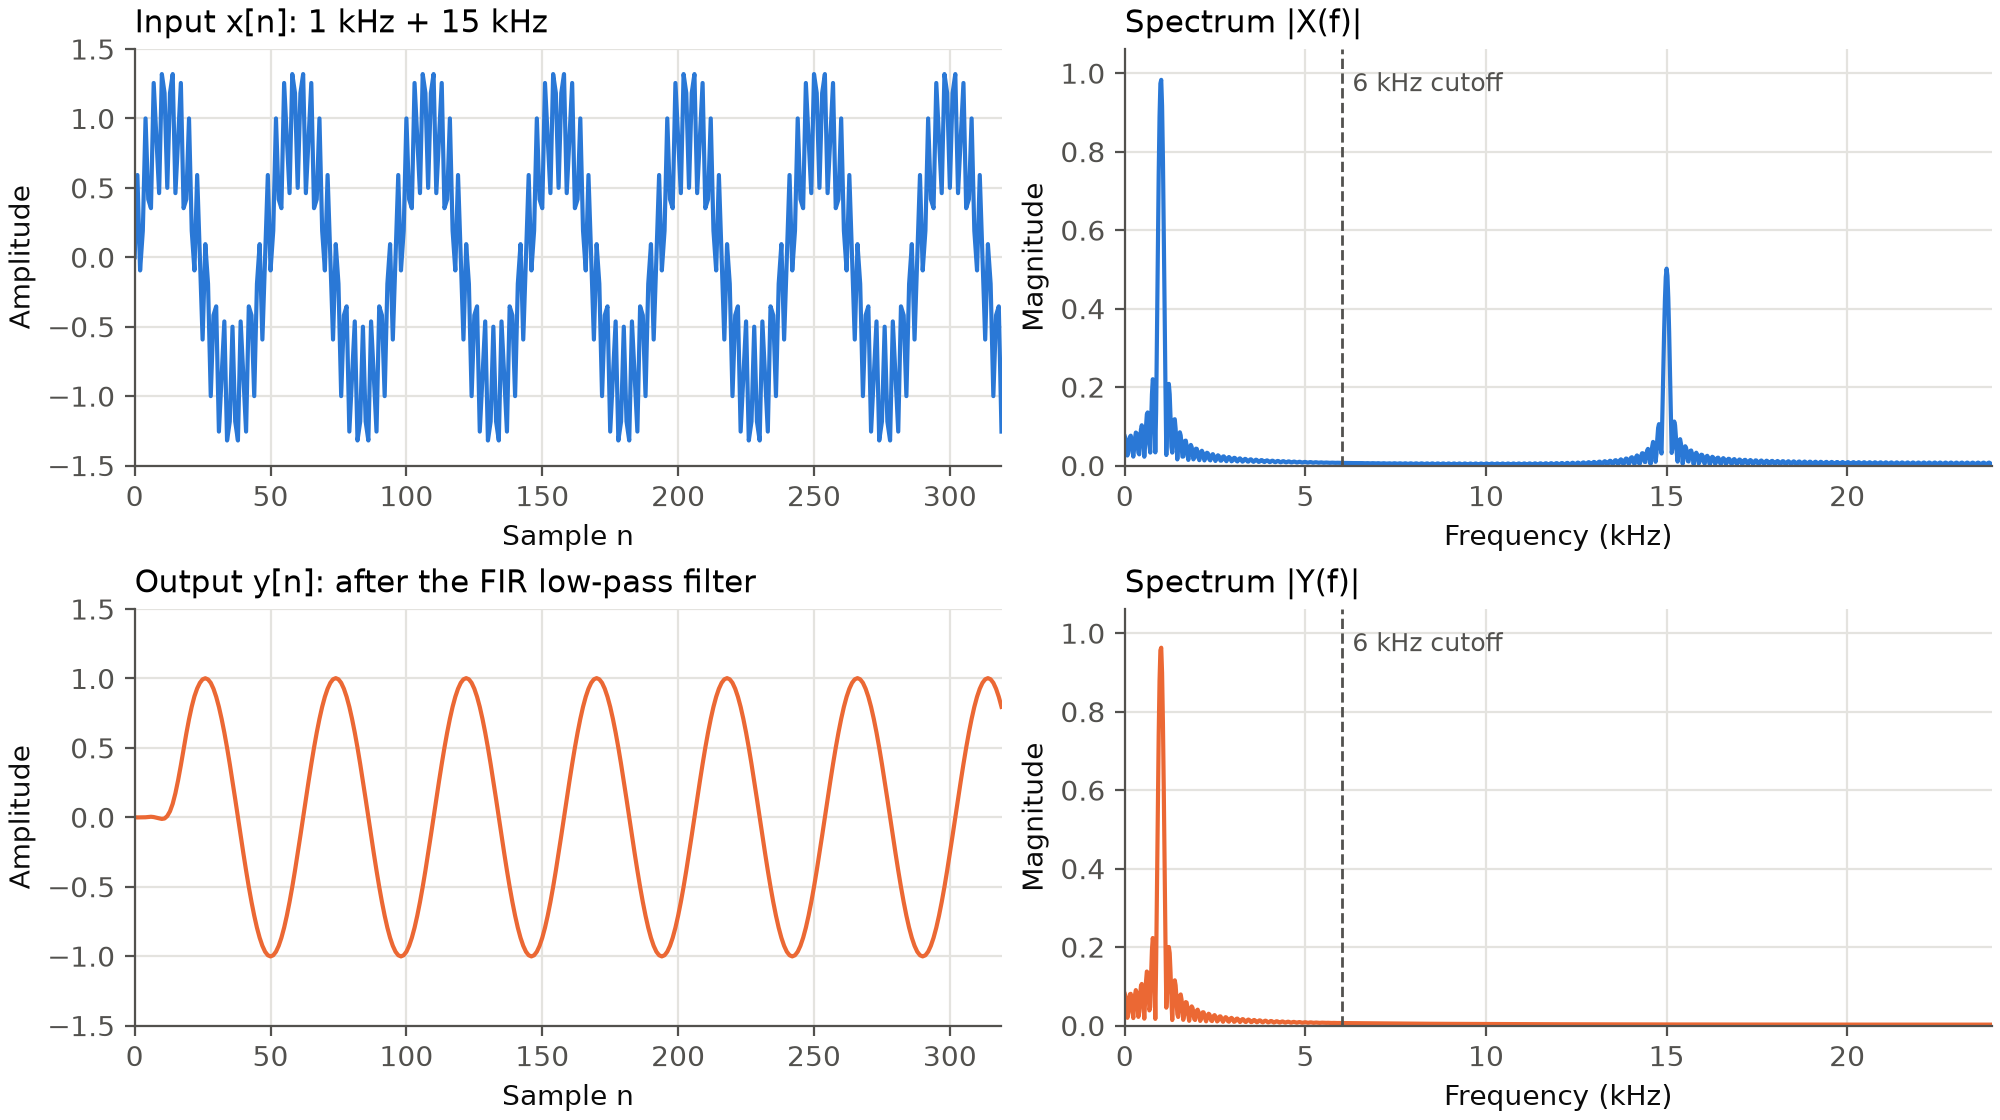
\includegraphics[width=\textwidth]{figures/fir_known_signal.png}
\caption{Known-signal test, measured on the board. Top: the input
         (1\,kHz + 15\,kHz). Bottom: the output of \texttt{arm\_fir\_f32()}.}
\label{fig:known}
\end{figure}

\subsection{Filter design for the accelerometer}

A hand on the board or a tap on the table makes short spikes in the
acceleration. The slow motion of the board is below a few hertz. I chose a
sample rate of 50\,Hz and a cutoff of 5\,Hz.

The script \texttt{design\_fir.py} designs the filter with
\texttt{scipy.signal.firwin()} and a Hamming window. This is the same method
as MATLAB \texttt{fir1()}. For the lecture filter, both give the same
coefficients within $4 \times 10^{-11}$. The script prints the coefficients
as a C array in time-reversed order, and it checks the gain:

\begin{table}[h]
\centering
\caption{Accelerometer filter: 29 taps, $f_s = 50$\,Hz, cutoff 5\,Hz.}
\begin{tabular}{@{}lc@{}}
\toprule
Frequency & Gain \\
\midrule
0\,Hz (gravity, slow tilt) & 0.00\,dB \\
5\,Hz (cutoff)             & $-6.06$\,dB \\
10\,Hz                     & $-63.97$\,dB \\
\midrule
Group delay                & 14 samples = 280\,ms \\
\bottomrule
\end{tabular}
\end{table}

For \texttt{fir1()} and \texttt{firwin()}, the cutoff is the $-6$\,dB point,
not the $-3$\,dB point.

\subsection{Sampling the sensor}

\texttt{BSP\_ACCELERO\_Init()} sets the LSM6DSL to an output data rate of
52\,Hz and $\pm 2$\,g. \texttt{BSP\_ACCELERO\_AccGetXYZ()} gives the three axes
in mg. The program uses the Z axis. When the board lies flat, Z is about
1000\,mg (gravity).

The main loop reads the sensor every 20\,ms. It keeps a deadline and adds
20\,ms to the deadline, not to the current time. A late read thus does not
shift all later reads. The comparison uses a signed difference, so it stays
correct when \texttt{HAL\_GetTick()} wraps after 49.7 days.

\begin{lstlisting}[caption={50\,Hz sampling and block filtering (basic problem, \texttt{main.c}, user code block WHILE).}]
if ((int32_t)(HAL_GetTick() - next) >= 0) {
  next += 20;
  BSP_ACCELERO_AccGetXYZ(accel);
  accIn[k] = (float32_t)accel[2];
  k++;
  if (k == ACC_BLOCK_SIZE)
  {
    arm_fir_f32(&accFilter, accIn, accOut, ACC_BLOCK_SIZE);
    for ( int j = 0; j < ACC_BLOCK_SIZE; j++) {
      printf("%lu,%f,%f\n", n++, accIn[j], accOut[j]);
    }
    k = 0;
  }
}
\end{lstlisting}

A block has 25 samples, which is 0.5\,s. The filter has its own instance and
its own state buffer, separate from the known-signal test. The program prints
25 lines of about 28 bytes after each block. At 115200\,baud this takes about
60\,ms, which is three sample periods. The deadline catches up after the
print, but three reads then come back to back. At 1\,Mbaud the print takes
about 7\,ms, so I raised USART1 to 1\,Mbaud. This rate divides exactly from
the 80\,MHz clock of USART1 and from the 48\,MHz clock of the ST-LINK.

\subsection{Results}

\texttt{plot\_acc.py} records 10\,s (500 samples) and draws
Figure~\ref{fig:acc}. I tapped the table twice during the recording.

\begin{figure}[h]
\centering
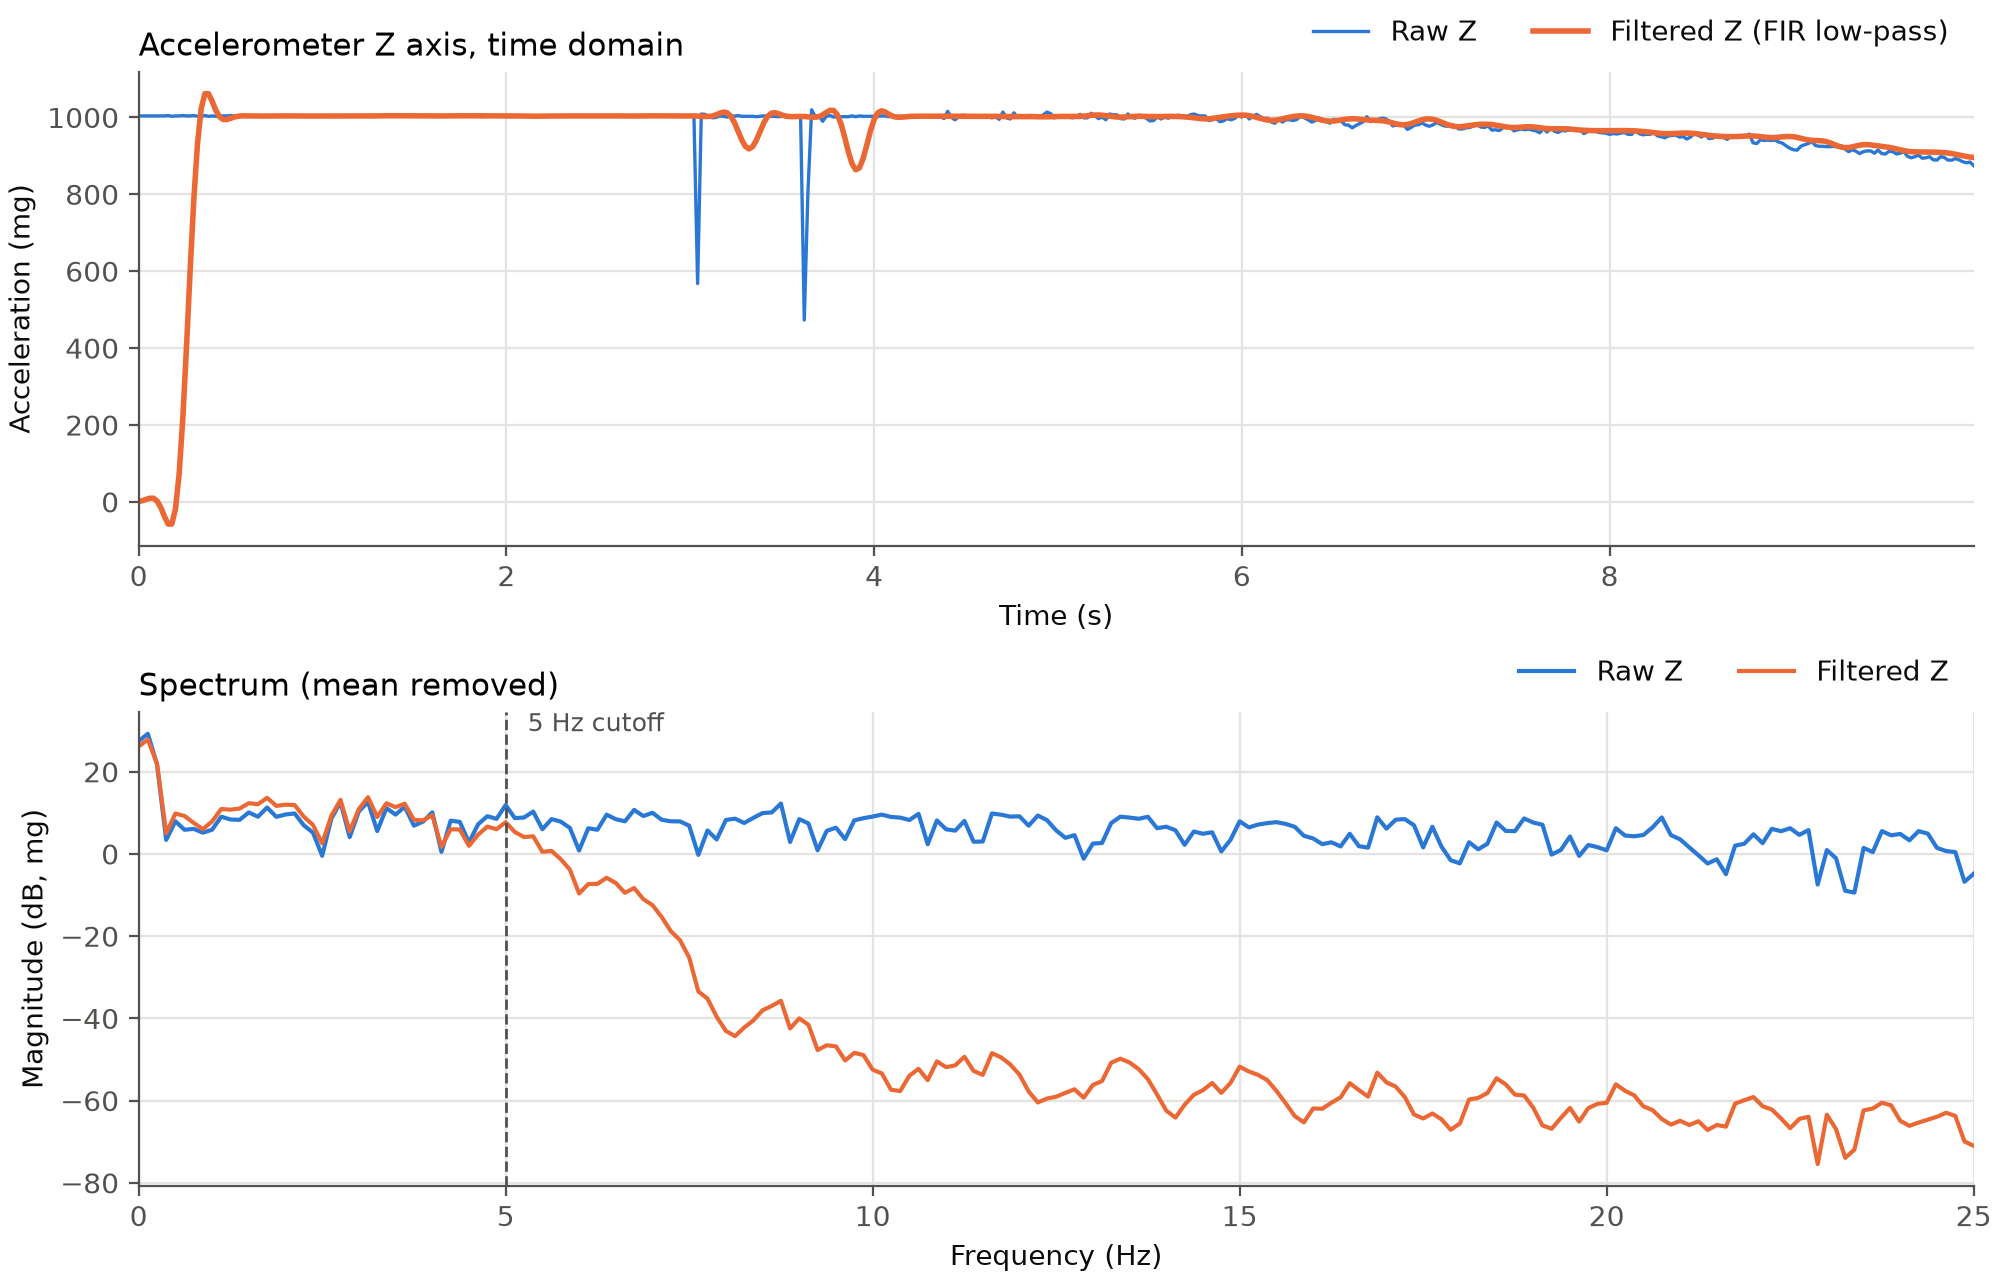
\includegraphics[width=\textwidth]{figures/acc_z.png}
\caption{Basic problem: Z acceleration before and after the filter. Top:
         time domain. Bottom: amplitude spectrum with the mean removed.}
\label{fig:acc}
\end{figure}

\begin{itemize}
  \item \textbf{Correctness.} I ran \texttt{scipy.signal.lfilter()} on the
        raw column with the same coefficients. The board output agrees within
        $2.3 \times 10^{-4}$\,mg on all 500 samples. The capture has 20 block
        boundaries, so this also proves that the state buffer carries the
        history from block to block.
  \item \textbf{Noise.} In a quiet second, the standard deviation of Z falls
        from 0.57\,mg to 0.22\,mg.
  \item \textbf{Spikes.} The taps reach 473\,mg in the raw data. The filtered
        signal goes down only to 864\,mg. The filter spreads each spike over
        about 0.5\,s, and it rings a little after it.
  \item \textbf{Spectrum.} The two curves are equal below 5\,Hz. Above about
        8\,Hz the filtered spectrum is 50 to 70\,dB lower.
  \item \textbf{Start and delay.} The filtered curve starts at 0 and rises to
        1000\,mg in the first 0.56\,s (28 samples), because the state starts
        at zero. Each filtered dip comes 280\,ms after its spike.
\end{itemize}

% =========================================================================
\section{Option Problem 1: Three Tasks with CMSIS-RTOS2}

\subsection{Design}

The option problem uses a separate CubeMX project in \texttt{lab7/rtos/}. It
starts from a copy of \texttt{lab7.ioc} and shares \texttt{lab7/ThirdParty/}.
The basic project stays unchanged.

\begin{figure}[h]
\centering
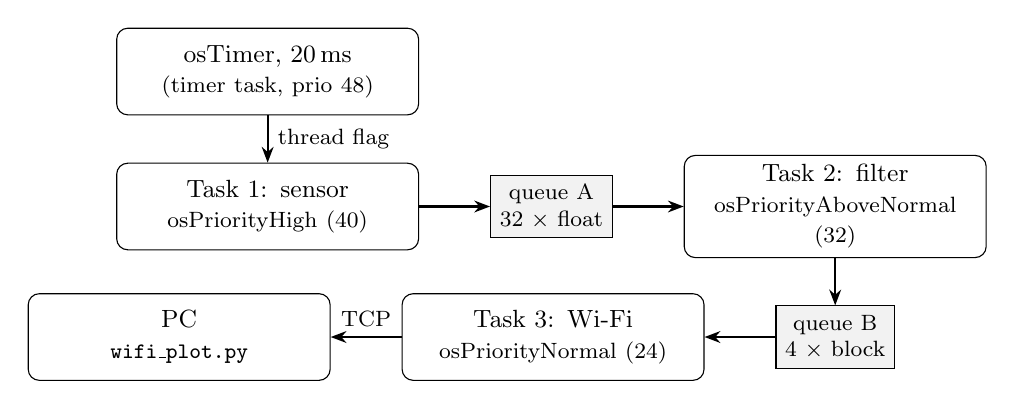
\begin{tikzpicture}[
    node distance=6mm and 9mm,
    box/.style={draw, rounded corners, align=center, minimum height=11mm,
                text width=36mm, font=\small},
    q/.style={draw, align=center, minimum height=7mm, font=\footnotesize,
              fill=black!5},
    arr/.style={-{Stealth[length=2mm]}, thick}]
  \node[box] (tmr) {osTimer, 20\,ms\\\footnotesize(timer task, prio 48)};
  \node[box, below=of tmr] (t1) {Task 1: sensor\\\footnotesize osPriorityHigh (40)};
  \node[q, right=of t1] (qa) {queue A\\32 $\times$ float};
  \node[box, right=of qa] (t2) {Task 2: filter\\\footnotesize osPriorityAboveNormal (32)};
  \node[q, below=of t2] (qb) {queue B\\4 $\times$ block};
  \node[box, left=of qb] (t3) {Task 3: Wi-Fi\\\footnotesize osPriorityNormal (24)};
  \node[box, left=of t3] (pc) {PC\\\footnotesize\texttt{wifi\_plot.py}};
  \draw[arr] (tmr) -- node[right, font=\footnotesize] {thread flag} (t1);
  \draw[arr] (t1) -- (qa);
  \draw[arr] (qa) -- (t2);
  \draw[arr] (t2) -- (qb);
  \draw[arr] (qb) -- (t3);
  \draw[arr] (t3) -- node[above, font=\footnotesize] {TCP} (pc);
\end{tikzpicture}
\caption{Tasks, timer and queues. A block holds the start index $n_0$, 25 raw
         samples and 25 filtered samples.}
\label{fig:design}
\end{figure}

\begin{itemize}
  \item \textbf{Task 1 (sensor)} has the highest priority, because it has the
        strictest timing. It reads one sample when the timer triggers it.
  \item \textbf{Task 2 (filter)} collects 25 samples, runs
        \texttt{arm\_fir\_f32()} and puts the raw and the filtered block into
        queue~B.
  \item \textbf{Task 3 (Wi-Fi)} has the lowest priority. A Wi-Fi send takes a
        long and variable time, and no other task waits for it.
\end{itemize}

Each queue decouples a fast producer from a slower consumer. The producers put
items with a timeout of 0. A full queue therefore never blocks a
higher-priority task. Instead, the producer counts the lost item:
\texttt{droppedSamples} for queue~A and \texttt{droppedBlocks} for queue~B.
The Wi-Fi task sends both counters every 10\,s.

\subsection{RTOS configuration}

\begin{table}[h]
\centering
\caption{FreeRTOS settings in CubeMX.}
\begin{tabular}{@{}lp{9.5cm}@{}}
\toprule
Setting & Value and reason \\
\midrule
Interface              & CMSIS\_V2 \\
HAL timebase           & TIM6. FreeRTOS uses SysTick for its own tick. \\
\texttt{TOTAL\_HEAP\_SIZE} & 32768 bytes for three task stacks, two queues and the timer \\
Task stacks            & 512, 512 and 1024 words. \texttt{printf()} with \texttt{\%f} needs more than the default 128 words. \\
\texttt{CHECK\_FOR\_STACK\_OVERFLOW} & Option 2, so an overflow stops the program and does not corrupt memory \\
\texttt{USE\_NEWLIB\_REENTRANT} & Enabled. Each task gets its own C library state for \texttt{printf()}. \\
\texttt{TIMER\_TASK\_PRIORITY} & 48 (osPriorityRealtime) instead of 2, see below \\
\bottomrule
\end{tabular}
\end{table}

An osTimer callback does not run in an interrupt. It runs in the FreeRTOS
timer service task. CubeMX gives this task the priority 2, which is below all
three of my tasks (24, 32 and 40). With that default, a busy Wi-Fi task delays
the timer callback, and the highest-priority task wakes up late. With
priority 48, the callback runs as soon as the timer expires. The callback only
sets a flag, so this priority costs almost no CPU time.

\subsection{Task 1: timer-triggered sensor reads}

\begin{lstlisting}[caption={Timer callback and sensor task (\texttt{rtos/Core/Src/main.c}, comments shortened).}]
void SampleTimerCallback(void *argument)
{
  osThreadFlagsSet(sensorTaskHandle, 0x01);
  sensorTickcounter++;
}

void StartSensorTask(void *argument)
{
  for(;;)
  {
    osThreadFlagsWait(0x01, osFlagsWaitAny, osWaitForever);
    int16_t xyz[3];
    BSP_ACCELERO_AccGetXYZ(xyz);
    sampleCount++;
    float32_t zValue = (float32_t)xyz[2];
    if (osMessageQueuePut(rawZQueueHandle, &zValue, 0, 0) != osOK) {
      droppedSamples++;
    }
  }
}
\end{lstlisting}

The I2C read happens in the task, not in the callback. Thread flags do not
count. If the timer fires twice before the task waits again, the task wakes
only once, and nothing reports the lost trigger. To detect this case, the
callback counts the triggers and the task counts the samples. A test version
printed both counters every 50 samples:

\begin{lstlisting}[style=plain,basicstyle=\ttfamily\scriptsize,caption={Test of task 1 (board flat on the table).}]
Sample Count: 50, Sensor Tick Counter: 50, Z Value: 1002, Elapsed Time: 1001 ms
Sample Count: 100, Sensor Tick Counter: 100, Z Value: 1001, Elapsed Time: 1000 ms
Sample Count: 150, Sensor Tick Counter: 150, Z Value: 1003, Elapsed Time: 1000 ms
...
Sample Count: 450, Sensor Tick Counter: 450, Z Value: 1003, Elapsed Time: 1000 ms
\end{lstlisting}

50 samples take 1000\,ms, so the rate is exactly 50\,Hz. The two counters are
always equal, so no trigger was lost. The first line includes the start-up
time.

The value goes into queue~A as \texttt{float32\_t}. The queue copies
\texttt{sizeof(float32\_t)} = 4 bytes from the given address. A pointer to the
\texttt{int16\_t} value would copy 2 bytes of the sample and 2 bytes of the
stack after it.

\subsection{Task 2: filter}

\begin{lstlisting}[caption={Filter task (comments and old test code removed).}]
osMessageQueueGet(rawZQueueHandle, &accIn[k], NULL, osWaitForever);
if (k == ACC_BLOCK_SIZE - 1) {
  arm_fir_f32(&accFilter, accIn, accOut, ACC_BLOCK_SIZE);
  AccDataBlock block;
  block.n0 = n;
  memcpy(block.raw, accIn, ACC_BLOCK_SIZE * sizeof(float32_t));
  memcpy(block.filt, accOut, ACC_BLOCK_SIZE * sizeof(float32_t));
  if (osMessageQueuePut(accDataQueueHandle, &block, 0, 0) != osOK) {
    printf("Failed to put block into queue\n");
    droppedBlocks++;
  }
  n += ACC_BLOCK_SIZE;
  k = 0;
} else {
  k++;
}
\end{lstlisting}

The blocking \texttt{osMessageQueueGet()} sets the pace of the task, so the
task needs no delay. The queue copies the whole block (204 bytes). The Wi-Fi
task thus gets its own copy, and the filter task can overwrite
\texttt{accIn} and \texttt{accOut} at once.

Before I added Wi-Fi, the filter task printed each block over the UART.
\texttt{plot\_acc.py} recorded 1050 samples (21\,s) with no index gaps, and
the board output matched \texttt{lfilter()} within
$2.6 \times 10^{-4}$\,mg (Figure~\ref{fig:rtosuart}).

\begin{figure}[h]
\centering
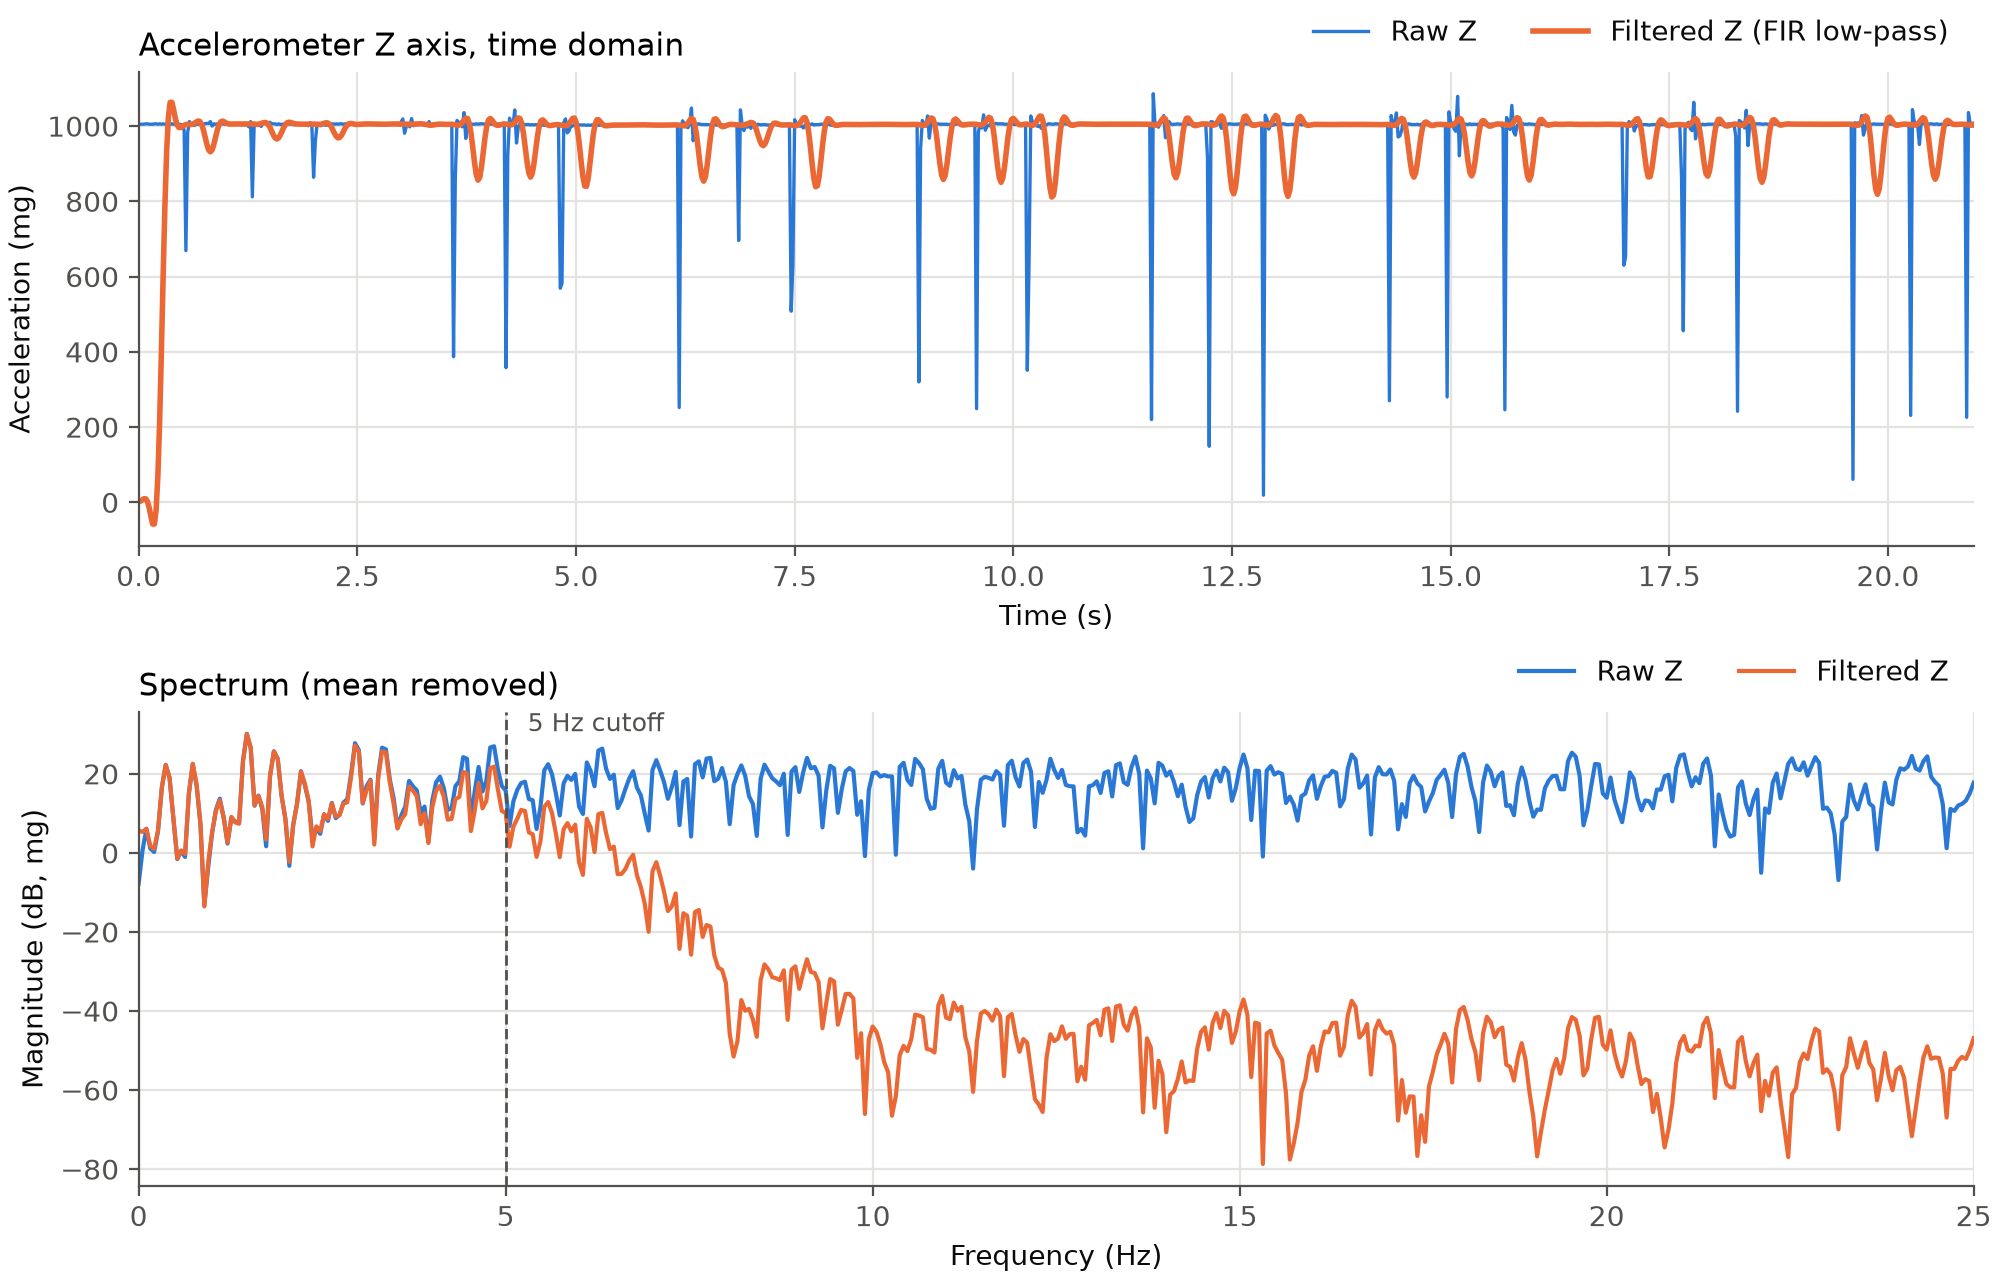
\includegraphics[width=\textwidth]{figures/rtos_acc_z.png}
\caption{RTOS version with UART output, before Wi-Fi: 21\,s with repeated
         taps.}
\label{fig:rtosuart}
\end{figure}

\subsection{Task 3: Wi-Fi}

The Wi-Fi task uses the ES-WiFi driver from the STM32CubeL4
\texttt{WiFi\_Client\_Server} example, as in lab~2. The driver talks to the
ISM43362 module over SPI3. It needs two interrupts: SPI3 and EXTI1, the
data-ready line of the module. The driver sets SPI3 up with its own handle
\texttt{hspi}, and it enables both interrupts itself. In CubeMX I enabled SPI3
only to get the HAL SPI driver into the build. I left the two interrupts off
in CubeMX. Otherwise CubeMX generates an \texttt{SPI3\_IRQHandler()} for its
own handle \texttt{hspi3}, and the transfers of the driver never complete. My
handlers in \texttt{stm32l4xx\_it.c} call \texttt{HAL\_SPI\_IRQHandler(\&hspi)}
and \texttt{HAL\_GPIO\_EXTI\_IRQHandler(GPIO\_PIN\_1)}.
\texttt{HAL\_GPIO\_EXTI\_Callback()} passes pin~1 to \texttt{SPI\_WIFI\_ISR()}.

The driver runs in its non-RTOS mode. It waits for the SPI flags in a busy
loop. This is acceptable because the Wi-Fi task has the lowest of the three
priorities. The sensor and filter tasks preempt it at any time, and only the
idle task loses CPU time.

At start, the task joins the access point, opens a TCP connection to the PC
(port 8002) and sends one test line. Each step prints its result, and a
failure stops the sequence. Then the task starts the sample timer. In the
loop, the task takes one block from queue~B, formats the 25 lines
\texttt{n,raw,filtered} into one buffer and sends it with one
\texttt{WIFI\_SendData()} call.

\begin{lstlisting}[caption={Wi-Fi task loop (error prints shortened, drop report left out).}]
osTimerStart(sampleTimerHandle, 20);
for(;;)
{
  AccDataBlock local_block;
  if (osMessageQueueGet(accDataQueueHandle, &local_block, NULL, osWaitForever) != osOK) {
    droppedBlocks++;
    continue;
  }
  size_t len = 0;
  for (int i = 0; i < ACC_BLOCK_SIZE; i++) {
    len += snprintf(buffer + len, sizeof(buffer) - len, "%lu,%f,%f\n",
                    local_block.n0 + i, local_block.raw[i], local_block.filt[i]);
  }
  if (WIFI_SendData(0, (const uint8_t*)buffer, len, &sent, 1000) != WIFI_STATUS_OK) {
    sendError++;
  } else if (sent != len) {
    sendError++;
  }
  /* every 20 blocks: send "# dropped=<samples> blocks=<blocks>" */
}
\end{lstlisting}

A block is 630 to 725 bytes. The driver cuts any send above 1200 bytes without
an error, so the task compares \texttt{sent} with \texttt{len}. One send per
block costs one Wi-Fi command every 0.5\,s.

\subsection{PC side}

\texttt{wifi\_plot.py} is a TCP server on port 8002. A thread receives the
data and splits it into lines. TCP is a byte stream, so one receive can hold
half a line or many lines. The plot shows the last 10\,s of raw and filtered
Z. The time axis is the board's sample index divided by 50\,Hz, not the
arrival time, because the samples arrive in bursts of 25. The title shows the
number of samples, the number of index gaps and the number of bad lines.
Lines that start with \texttt{\#} go to the terminal. At the end, the program
saves a CSV file in the format of \texttt{plot\_acc.py}.

I tested the receiver on the PC first. A test client replayed a recorded CSV
in blocks, with a block split in the middle of a line, a missing block, a bad
line and a comment line. The receiver joined the split line, reported one
gap, counted one bad line and printed the comment.

\subsection{Results}

The board joined the access point and got the address 192.168.50.102 in the
same network as the PC. Before I moved the timer start, the sensor and filter
tasks ran while the Wi-Fi task connected:

\begin{lstlisting}[style=plain,caption={Serial output during the Wi-Fi start (timer started at boot, filter task printing the drop counter, network name removed).}]
BEGIN WIFI
WIFI_Init OK
Connecting to SSID: <lab network>
# Dropped Samples: 0
WIFI_Connect OK
Opening TCP client connection to 192.168.50.178:8002
# Dropped Samples: 0
WIFI_OpenClientConnection OK
Sending data...
WIFI_SendData OK, sent 30 bytes
\end{lstlisting}

\texttt{WIFI\_Connect()} takes several seconds. During this time queue~A lost
no sample. The sensor and filter tasks preempted the busy-waiting Wi-Fi task,
as the priorities intend.

Figure~\ref{fig:wifi} shows the final version, recorded on the PC from the
Wi-Fi stream. It has 1725 samples (34.5\,s) with no index gap and no bad
line. The filtered column agrees with \texttt{lfilter()} on the received raw
column within $2.3 \times 10^{-4}$\,mg. The filter on the board and the
transfer over Wi-Fi are therefore both correct.

\begin{figure}[h]
\centering
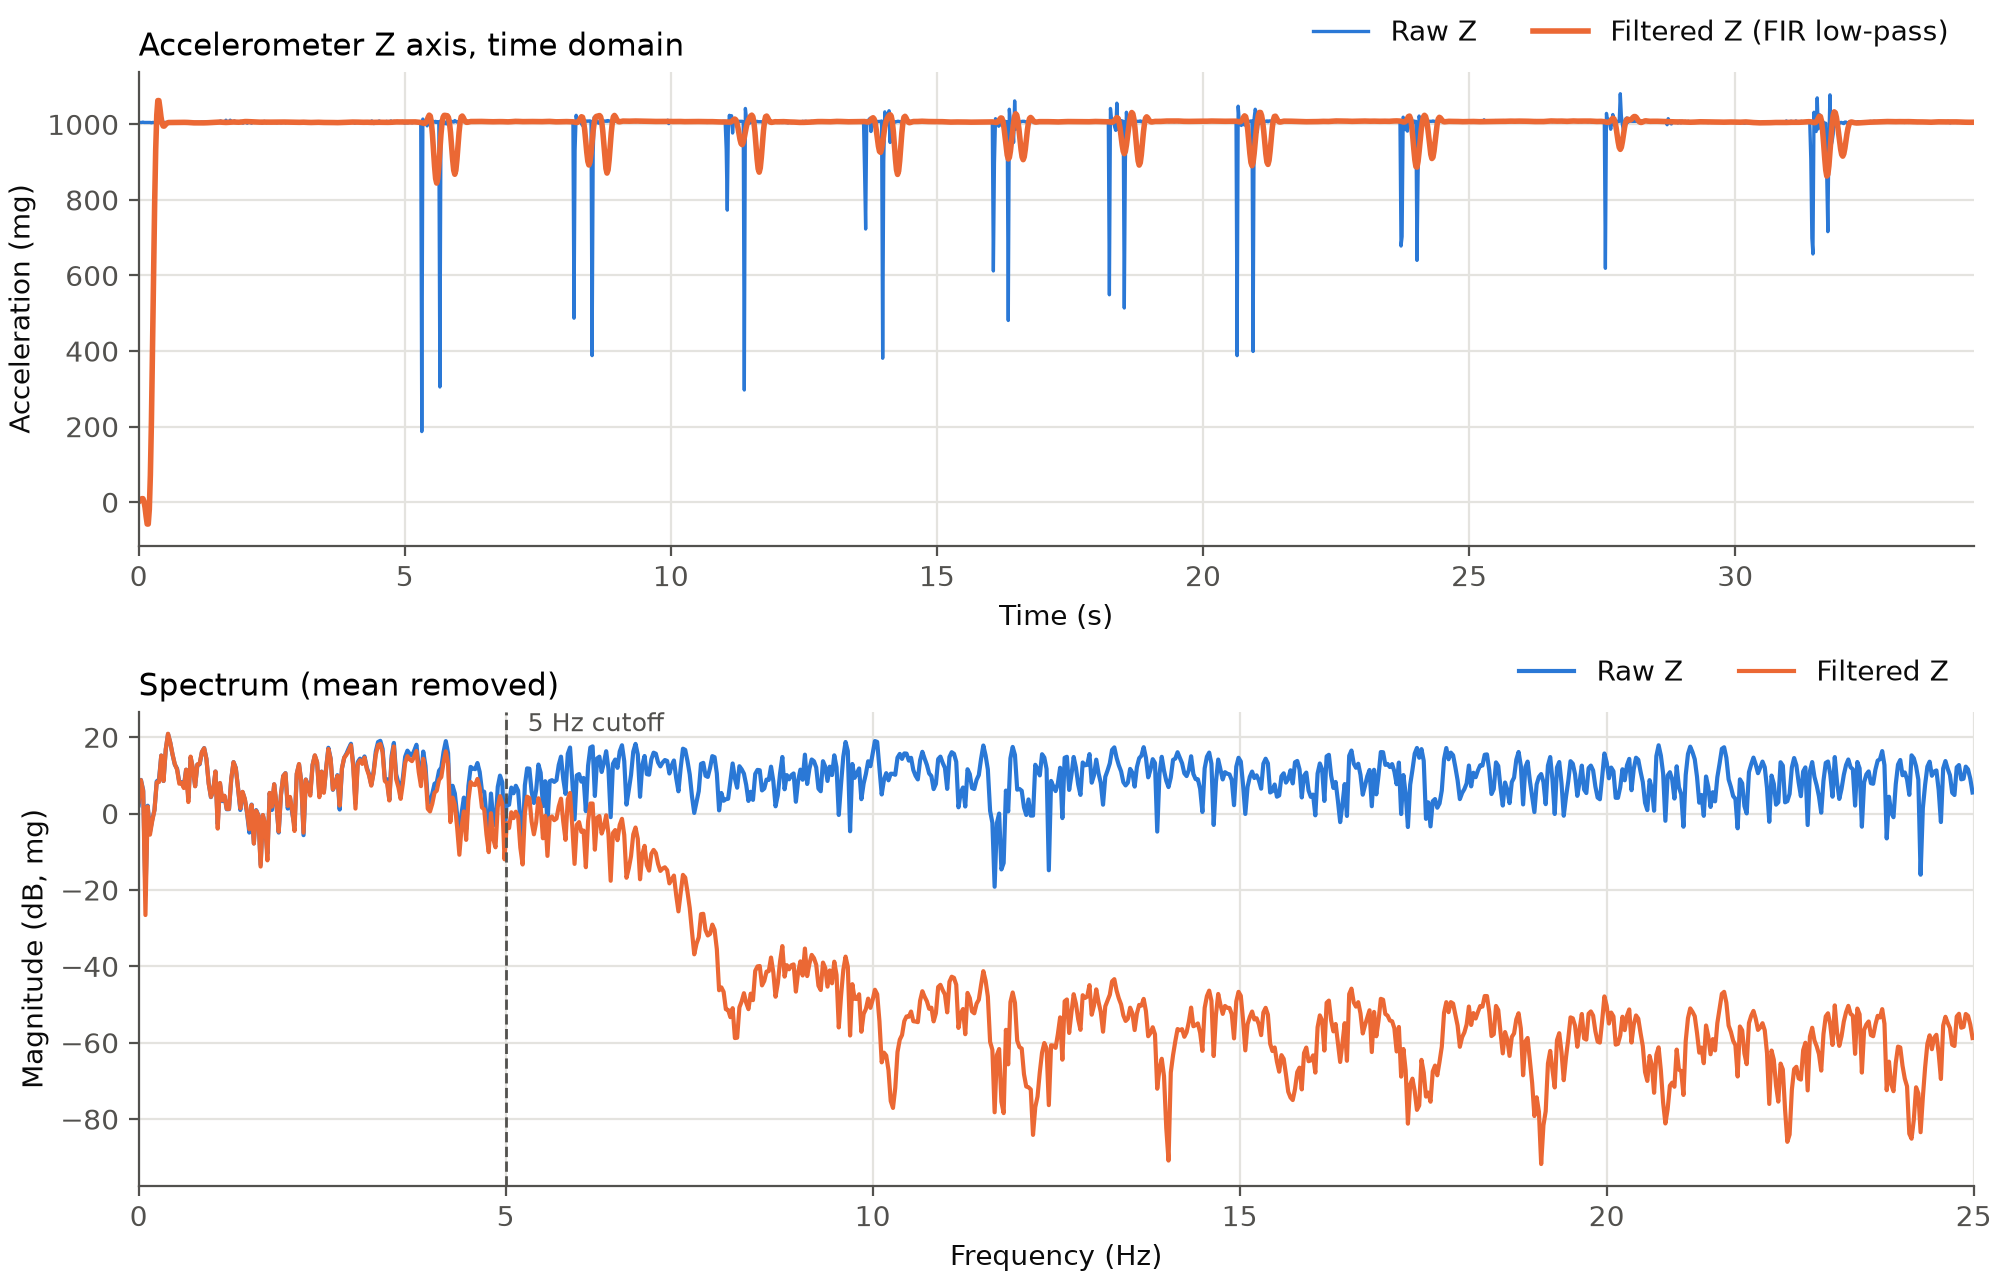
\includegraphics[width=\textwidth]{figures/wifi_acc_z.png}
\caption{Option problem: raw and filtered Z received over Wi-Fi, with taps
         every few seconds.}
\label{fig:wifi}
\end{figure}

\subsection{Discussion}

\paragraph{Start-up drops.}
In the first Wi-Fi version, the timer started at boot. Queue~B holds four
blocks, so it was full 2\,s after boot, while the Wi-Fi task was still
connecting. The filter task dropped the next 11 blocks. The PC received
samples 0 to 99, then a gap to 375, and the board reported
\texttt{blocks=11}. $11 \times 25 = 275 = 375 - 100$, so the counter on the
board and the gap on the PC agree exactly. Now the Wi-Fi task starts the
timer after the connection works, and the stream starts at $n = 0$ with no
gap.

\paragraph{Send errors that lose no data.}
In the same run, 18 sends reported a failure. The driver prints
\texttt{Send Data command failed} (\texttt{es\_wifi.c}, line 2311) when the
reply of the module after the data does not contain \texttt{OK}. But the PC
received every block after the start-up gap, once and complete. The error is
in the acknowledgement, not in the data. I checked one possible cause: the
driver pads odd-length sends with one byte. 79 of the 129 blocks had an odd
length, but only 18 sends failed, so the length is not the cause. The cause
is still open. The sequence check on the PC is the evidence that no data was
lost. A design that needs every block must not resend on this error, because
the PC already has the data. It needs a sequence number in each block, as
here, and the PC must drop duplicates.

\paragraph{Latency.}
A sample reaches the PC after up to 0.5\,s for the block, plus the
group delay of 280\,ms, plus the Wi-Fi transfer. The block size sets the
trade-off: smaller blocks reduce the delay, but they need more Wi-Fi
commands per second. Lab~2 showed that the send rate of this module is
limited.

\paragraph{Why the queues, and not shared variables.}
Without queue~B, the Wi-Fi task would read \texttt{accIn} and \texttt{accOut}
while the filter task overwrites them, and lines from two blocks would mix. A
draft of the Wi-Fi loop had this bug, and a code review found it before I
flashed it. The queue copies the data, so each task owns its own buffer and
needs no mutex.

% =========================================================================
\section{Problems Encountered}

Table~\ref{tab:problems} lists the problems in the order they occurred. The
rows ``Found before flashing'' come from code reviews. They never reached the
board.

\begin{table}[H]
\centering
\caption{Problems, their symptoms and causes.}
\label{tab:problems}
\footnotesize
\begin{tabular}{@{}>{\raggedright\arraybackslash}p{2.9cm}%
                  >{\raggedright\arraybackslash}p{5.0cm}%
                  >{\raggedright\arraybackslash}p{7.3cm}@{}}
\toprule
Problem & Symptom & Cause and fix \\
\midrule
Library not found &
  CMake cannot find the CMSIS-DSP files. &
  CMake does not expand \texttt{\~{}} in paths. I copied the files into
  \texttt{ThirdParty/} and used \texttt{\$\{CMAKE\_CURRENT\_SOURCE\_DIR\}}. \\
No float output &
  \texttt{(int)result[0]*1000} printed 3000 for 3.75. &
  The cast binds before the multiplication. newlib-nano has no
  \texttt{\%f}, so I added \texttt{-u \_printf\_float}. \\
Failure test said ``Success'' &
  The log showed Success after the coefficient change. &
  The log held the old program, which ran until the new one was flashed. The
  next reset printed 25.16\,dB, Failure. \\
No sensor output &
  Only the FIR dump appeared. &
  The sensor code was in \texttt{USER CODE 3}, which ends after the closing
  brace of the loop. It never ran. \\
1\,Mbaud not offered &
  The VS Code Serial Monitor has no 1\,Mbaud setting. &
  \texttt{python -m serial.tools.miniterm COM3 1000000}. \\
Debugger does not start &
  ``error 138'' dialog. The GDB server log says TCP port 61234 is not
  available. &
  Windows reserves the ports 61186--61285 for Hyper-V/WSL. \texttt{launch.json}
  sets \texttt{serverPort} to 3333. \\
Timer task priority &
  No symptom. Found in \texttt{FreeRTOSConfig.h}. &
  The timer task had priority 2, below all tasks. I set it to 48. \\
Found before flashing &
  Queue item of 4 bytes from an \texttt{int16\_t}. \texttt{osDelay(1000)} in
  the filter loop. \texttt{osMessageQueueGet()} with a \texttt{NULL} buffer. &
  Wrong data, 49 of 50 samples dropped, and a loop that never waits: CMSIS
  returns \texttt{osErrorParameter} at once for a \texttt{NULL} buffer. All
  three fixed. \\
Wi-Fi driver does not build &
  \texttt{stm32l4xx\_hal\_spi.h} missing. &
  The HAL SPI driver was not in the project. I enabled SPI3 in CubeMX, with
  its interrupts off. \\
Gap at start &
  PC: samples 0--99, then 375. Board: \texttt{blocks=11}. &
  Queue~B was full while Wi-Fi connected. The timer now starts after the
  connection. \\
Send errors &
  \texttt{Send Data command failed} on 18 sends. &
  The data arrived anyway (no gap). The cause is open, see the discussion. \\
\bottomrule
\end{tabular}
\end{table}

% =========================================================================
\section{Conclusion}

The CMSIS-DSP FIR filter runs on the Cortex-M4F with the hardware FPU. The
known-signal test gives an SNR of 142.6\,dB against the MATLAB reference. A
deliberate error of one coefficient drops it to 25.2\,dB, as a hand
calculation predicts. A 29-tap, 5\,Hz low-pass filter then smooths the Z
acceleration at 50\,Hz. Its output agrees with SciPy within
$2.3 \times 10^{-4}$\,mg, across all block boundaries.

For option problem~1, three CMSIS-RTOS2 tasks share the work. A timer triggers
the sensor task at exactly 50\,Hz without a lost trigger. Queues carry the
data to the filter task and the Wi-Fi task, and counters on both queues show
every lost item. The PC receives and plots the raw and the filtered signal
with no gap, and the received data agrees with SciPy.

The main lesson is to make every loss visible. Thread flags, full queues and
Wi-Fi sends can all fail without an error. Counters on the board, together
with the sample index on the PC, showed the 11 lost blocks at start-up and
proved that the 18 send errors lost no data.

\end{document}
